% --------------------------------------------
% LaTeX-Beamer-Vorlage des Arbeitsbereichs AmP
% Autor: Dipl.-Ing. Arthur Seibel ------------
% --------------------------------------------
%
% ----------------------------
% --------- Pr�ambel ---------
% ----------------------------
%
\documentclass[
%10pt
%11pt
%12pt
]{beamer} % Dokumentklasse
%\documentclass[draft]{beamer} % Entwickler-Modus in dem das File schneller kompiliert wird
%\documentclass[handout]{beamer} % Zum Ausdrucken besser geeignete Version der Folien
%\documentclass{article} % Artikel-Version; Funktioniert nur, wenn man zus�tzlich das Paket beamerarticle mittels 
%\usepackage{beamerarticle} % einbindet.
%
\usepackage{pgfplots} % Chemical
\usepackage[ansinew]{inputenc} % erweiterter Eingabezeichensatz (z.B. Sonderzeichen, Umlaute, etc.)
\usepackage[T1]{fontenc} % erweiterter T1 Zeichenvorrat
%\usepackage[ngerman]{babel} % Deutsche Trennregeln
\usepackage{amsmath} % Matheumgebung
\usepackage{mathtools} % erweiterte Matheumgebung
\usepackage{dsfont} % f�r mathematische Mengensymbole
\usepackage{amssymb} % Symbolumgebung
\usepackage{lmodern} % Serifenlose Schrift
\usepackage{tikz}    % TikZ Pictures 
\usepackage{graphics} % Einbindung von Grafiken in PS, PDF und JPG
\usepackage{pifont}
\usepackage{url} % Internetlinks eingeben �ber \url{http://www.tu-harburg.de}
\usepackage{listings}             % Include the listings-package
%
\usepackage{hyperref}
\usetheme{Madrid} % Pr�senthationsthema
\usecolortheme[RGB={45,198,214}]{structure} % Farbthema
\definecolor{tuhh}{RGB}{45,198,214} % Eigene Farbdefinition 
\useinnertheme{rounded} % Inneres Thema


%
% ----- Metainformationen -----
%


\setbeamercovered{transparent} % Transparente Overlays
\setbeamertemplate{frametitle}
{%
\vspace{-0.12ex}
\begin{beamercolorbox}[wd=\paperwidth,dp=0ex,ht=4ex,sep=0.5ex,colsep*=0pt]{frametitle}%
    \usebeamerfont{frametitle} \strut \insertframetitle  \hfill \raisebox{-1.7ex}[0pt][-\ht\strutbox ]{
\documentclass[•]{standalone}
\usepackage{tikz}

\begin{document}
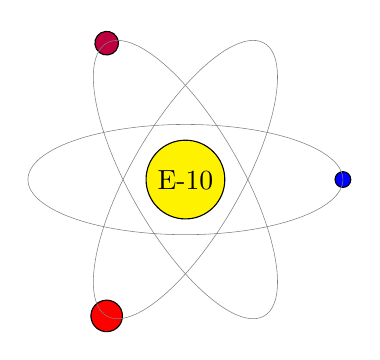
\begin{tikzpicture}


\draw[fill=blue] (2,0) circle(.1);
\draw[help lines] (0,0)ellipse(2 and .7);
\begin{scope}[rotate=60]
\draw[fill=red] (-2,0) circle(.2);
\draw[help lines] (0,0)ellipse(2 and .7);
\end{scope}
\begin{scope}[rotate=120]
\draw[fill=purple] (2,0) circle(.15);
\draw[help lines] (0,0)ellipse(2 and .7);
\end{scope}
\draw[fill=yellow] (0,0)circle(.5)node{E-10};
\end{tikzpicture}
\end{document}}
    \end{beamercolorbox}%
 }%
%
\title[simulation of a chemical reaction]{Simulation of chemical reaction kinetics}
\author[Lars Schiller]{Lars Schiller}
\institute[E-10]{E-10-Simulation GmbH}
\date{\today}
% Alternativ kann mittels 
%\date{\today} % auch das aktuelle Datum eingetragen werden.
\titlegraphic{\includegraphics[height=4cm]{inst_logo_title.pdf}} % Logo unten zentriert
%
%% Inhaltsverzeichnis vor jedem Teilabschnitt:
%\AtBeginSection[]
%{
%  \begin{frame}<beamer>[noframenumbering]
%    \frametitle{�bersicht}
%    \tableofcontents[currentsection] % , subsection
%  \end{frame}
%}
%
% ---------- Dokument ----------
% ------------------------------
%
\begin{document}
%
%---------------------------------------
\begin{frame}%[noframenumbering]
\titlepage
\end{frame}


\begin{frame}
\frametitle{Problem description and mathematical model}

\begin{center}
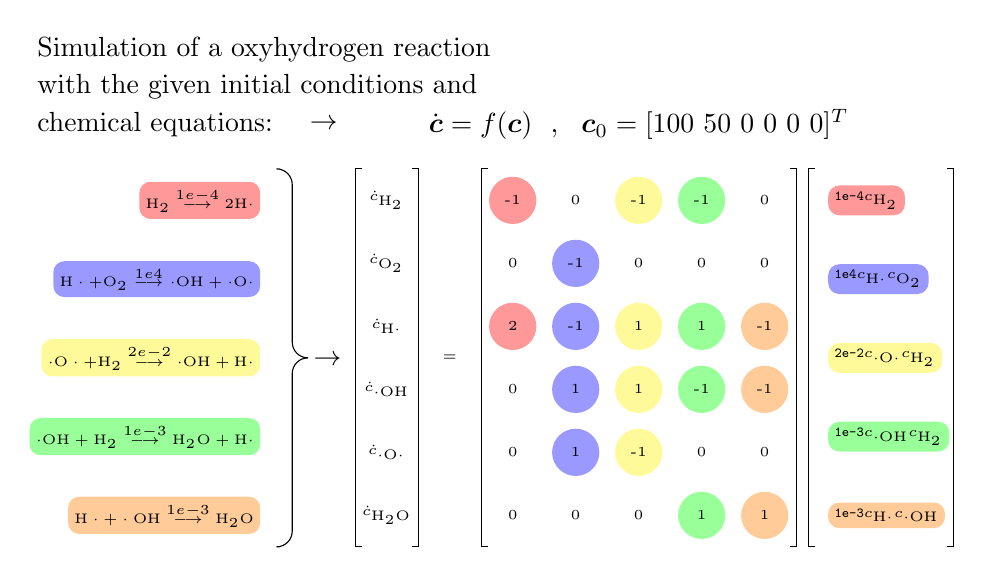
\begin{tikzpicture}[scale=.8]
\path (-5.7,1.4)node[right]{Simulation of a oxyhydrogen reaction};
\path (-5.7,.8)node[right]{with the given initial conditions and};
\path (-5.7,.2)node[right,align = right]{ chemical equations:};
\path (-1,.2)node{$\rightarrow$};

\path (4,.2)node{$\dot{\boldsymbol{c}} = f(\boldsymbol{c})~~,~~ \boldsymbol{c}_0 = [100~50~0~0~0~0]^T$};


\begin{tiny}
\path(-2,-1)node[left,align=right,draw = none, fill=red!40,rounded corners]{$\text{H}_2 \overset{1e-4}{\longrightarrow}2\text{H}\cdot$};
\path(-2,-2.25)node[left,align=right,draw = none, fill=blue!40,rounded corners]{$\text{H}\cdot +\text{O}_2 \overset{1e4}{\longrightarrow} \cdot\text{OH} + \cdot\text{O}\cdot $};
\path(-2,-3.5)node[left,align=right,draw = none, fill=yellow!40,rounded corners]{$\cdot\text{O}\cdot +\text{H}_2 \overset{2e-2}{\longrightarrow} \cdot\text{OH} + \text{H}\cdot $};
\path(-2,-4.75)node[left,align=right,draw = none, fill=green!40,rounded corners]{$\cdot\text{OH}+\text{H}_2 \overset{1e-3}{\longrightarrow} \text{H}_2\text{O} + \text{H}\cdot $};
\path(-2,-6)node[left,align=right,draw = none, fill=orange!40,rounded corners]{$\text{H}\cdot + \cdot\text{OH} \overset{1e-3}{\longrightarrow} \text{H}_2\text{O}$};

\draw[rounded corners = .2cm] (-2+.3,-.5)--(-2+.5,-.5)--(-2+.5,-3.5)--(-2+.7,-3.5);
\draw[rounded corners = .2cm]	(-2+.7,-3.5)--(-2+.5,-3.5)--(-2+.5,-6.5)--(-2+.3,-6.5);
\path (-2+.73,-3.54) node[right]{\normalsize{$\rightarrow$}};

\draw (-.4,-.5)--(-.5,-.5)--(-.5,-6.5)--(-.4,-6.5);
\draw (.4,-.5)--(.5,-.5)--(.5,-6.5)--(.4,-6.5);
\path (0,-1)node{$\dot{c}_{\text{H}_2}$};
\path (0,-2)node{$\dot{c}_{\text{O}_2}$};
\path (0,-3)node{$\dot{c}_{\text{H}\cdot}$};
\path (0,-4)node{$\dot{c}_{\cdot\text{OH}}$};
\path (0,-5)node{$\dot{c}_{\cdot\text{O}\cdot}$};
\path (0,-6)node{$\dot{c}_{\text{H}_2\text{O}}$};

\path(1,-3.5)node{$=$};

\draw (2-.4,-.5)--(2-.5,-.5)--(2-.5,-6.5)--(2-.4,-6.5);
\path (2,-1)node[draw = none,circle,fill=red!40,minimum height=.6cm]{-1};
\path (2,-2)node{0};
\path (2,-3)node[draw = none,circle,fill=red!40,minimum height=.6cm]{2};
\path (2,-4)node{0};
\path (2,-5)node{0};
\path (2,-6)node{0};

\path (3,-1)node{0};
\path (3,-2)node[draw = none,circle,fill=blue!40,minimum height=.6cm]{-1};
\path (3,-3)node[draw = none,circle,fill=blue!40,minimum height=.6cm]{-1};
\path (3,-4)node[draw = none,circle,fill=blue!40,minimum height=.6cm]{1};
\path (3,-5)node[draw = none,circle,fill=blue!40,minimum height=.6cm]{1};
\path (3,-6)node{0};

\path (4,-1)node[draw = none,circle,fill=yellow!40,minimum height=.6cm]{-1};
\path (4,-2)node{0};
\path (4,-3)node[draw = none,circle,fill=yellow!40,minimum height=.6cm]{1};
\path (4,-4)node[draw = none,circle,fill=yellow!40,minimum height=.6cm]{1};
\path (4,-5)node[draw = none,circle,fill=yellow!40,minimum height=.6cm]{-1};
\path (4,-6)node{0};

\path (5,-1)node[draw = none,circle,fill=green!40,minimum height=.6cm]{-1};
\path (5,-2)node{0};
\path (5,-3)node[draw = none,circle,fill=green!40,minimum height=.6cm]{1};
\path (5,-4)node[draw = none,circle,fill=green!40,minimum height=.6cm]{-1};
\path (5,-5)node{0};
\path (5,-6)node[draw = none,circle,fill=green!40,minimum height=.6cm]{1};

\path (6,-1)node{0};
\path (6,-2)node{0};
\path (6,-3)node[draw = none,circle,fill=orange!40,minimum height=.6cm]{-1};
\path (6,-4)node[draw = none,circle,fill=orange!40,minimum height=.6cm]{-1};
\path (6,-5)node{0};
\path (6,-6)node[draw = none,circle,fill=orange!40,minimum height=.6cm]{1};
\draw (6+.4,-.5)--(6+.5,-.5)--(6+.5,-6.5)--(6+.4,-6.5);

\draw (7.2-.4,-.5)--(7.2-.5,-.5)--(7.2-.5,-6.5)--(7.2-.4,-6.5);
\path(7,-1)node[right,align=left,draw = none, fill=red!40,rounded corners]{$\texttt{1e-4} c_{\text{H}_2} $};
\path(7,-2.25)node[right,align=left,draw = none, fill=blue!40,rounded corners]{$\texttt{1e4} c_{\text{H}\cdot} c_{\text{O}_2}$};
\path(7,-3.5)node[right,align=left,draw = none, fill=yellow!40,rounded corners]{$\texttt{2e-2} c_{\cdot\text{O}\cdot} c_{\text{H}_2} $};
\path(7,-4.75)node[right,align=left,draw = none, fill=green!40,rounded corners]{$\texttt{1e-3} c_{\cdot\text{OH}} c_{\text{H}_2} $};
\path(7,-6)node[right,align=left,draw = none, fill=orange!40,rounded corners]{$\texttt{1e-3} c_{\text{H}\cdot} c_{\cdot\text{OH}} $};
\def\b{8.5}
\draw (\b+.4,-.5)--(\b+.5,-.5)--(\b+.5,-6.5)--(\b+.4,-6.5);

\end{tiny}

\end{tikzpicture}
\end{center}

\end{frame}


\begin{frame}
\frametitle{Choice and description of suited numerical solvers}
\begin{itemize}
\item Since the problem is \textit{stiff}, we have to choose an implicit multi-step method to obtain a large domain of stability (A-stable).
\item Try \textit{Adams-Moulton}-method and \textit{BDF}-method with $k=1$ steps and a step size $h = \texttt{1e-2}$: 
\end{itemize}

\begin{equation}
\sum\limits_{j=0}^k a_j y_{n+j} = h \sum\limits_{j=0}^k b_j f_{n+j}
\end{equation}

\begin{columns}
\begin{column}{.48\textwidth}
\begin{center}
\textit{Adams-Moulton:}

\begin{tabular}{c|cc|cc}
$k$ & $a_0$ & $a_1$ & $b_0$ & $b_1$ \\
\hline
1 & -1 & 1 & 0.5 & 0.5 \\
\end{tabular}
$$
F(y_{n+1}) = y_n + \frac{h}{2}\left( f_{n} +  f_{n+1} \right) - y_{n+1}
$$

\end{center}
\end{column}
\begin{column}{.48\textwidth}
\begin{center}
\textit{BDF:}

\begin{tabular}{c|cc|cc}
$k$ & $a_0$ & $a_1$ & $b_0$ & $b_1$ \\
\hline
1 & -1 & 1 & 0 & 1 \\
\end{tabular}
$$
F(y_{n+1}) = y_n + h f_{n+1} - y_{n+1}
$$

\end{center}
\end{column}
\end{columns}
\end{frame}

\begin{frame}[fragile]
\frametitle{Implementation of the numerical solvers}

\begin{columns}
\begin{column}{.51\textwidth}
\lstset{language=Matlab}          % Set your language (you can change the language for each code-block optionally)
\begin{lstlisting}[frame = single]  % Start your code-block

% Classic Iteration Loop
while (n+k-1)*h < tend
  % Newton-method
  [...] % initializing 
  Fi = F(y(n+k-1));
  while norm(Fi) > tol
    [...] % calculate JFi
    yi(i+1) = yi(i)-JFi\Fi; 
    Fi = F(yi(i+1));
    i = i+1;
  end
  y(n+k) = yi(i);
  n = n+1;
end
\end{lstlisting}
\end{column}
\begin{column}{.45\textwidth}
To calculate the Jacobian:

$$
JF(y) = 
\begin{bmatrix}
\frac{\delta F(y)}{\delta y_1} & \cdots & \frac{\delta F(y)}{\delta y_N}
\end{bmatrix}
$$

$$\frac{\delta F(y)}{\delta y_i} = \frac{F(y+\hat{h}e_i) - F(y)}{\hat{h}} $$

\end{column}
\end{columns}
\end{frame}


\begin{frame}
\frametitle{comparison and evaluation of the numerical solvers}
\begin{center}
\includegraphics[width=.95\textwidth]{figures/Kombi.pdf}

\begin{tabular}{c|cccc|c}
method & fun eval & max NS & average NS & ct [sec] & $|\texttt{err}|$ \\
\hline
\texttt{A-M} & 91016 & 7 & 1.0145 & 4.0205 & 0.0347 \\
\texttt{BDF} & 80476 & 7 & 1.0068 & 5.7835 & 13.5788 \\
\texttt{ode15s} & 988 & - & - & 0.4859 & \texttt{ref} \\

\end{tabular}

\end{center}


\end{frame}

\end{document}
%
